%%%%%%%%%%%%%%%%%%%%%%%%%%%%%%%%%%%%%%%%%%%%%%%%%%%%%%%%%
%                 File: UV1310cdc.tex               	%
%                  Date: 10 Oct, 2015                	%
%                                                    	%
%   For submission to a OFC      						%
%                                                     	%
%   Technical paper about the results obtained with   	%
%   professor Wei Shi with tunable cascaded				%
%	contra-directional coupler				      		%
%	+ theorical analysis								%
%%%%%%%%%%%%%%%%%%%%%%%%%%%%%%%%%%%%%%%%%%%%%%%%%%%%%%%%%



\documentclass[letterpaper,10pt]{article}
\usepackage{osameet2}

\usepackage[utf8]{inputenc} %encoding of the input(this text file)
\usepackage[T1]{fontenc} 	%uses the right font encoding
\usepackage{lmodern,textcomp}		%makes font work for fontenc
\usepackage[french,english]{babel} %multiple languages
\selectlanguage{english}	%can switch to french later using this

\usepackage{ulem}
\usepackage{amsmath,amssymb}

\usepackage{graphicx,epsfig,epstopdf}

\usepackage{xcolor}
\newcommand\todo[1]{\textcolor{red}{#1}}
%\renewcommand\todo[1]{}  %activate to get rid of comments

\begin{document}

\title{O-band Silicon Photonic Bragg-Grating Multiplexers using UV Lithography}




\author{Jonathan St-Yves, Sophie Larochelle, and Wei Shi$^*$}
\address{Centre d'optique, photonique et laser (COPL) and Département de génie électrique, Université Laval, 2375 rue de la Terrasse, Québec (Québec), Canada, G1V 0A6}
%\email{jonathan.st-yves.1@ulaval.ca}
\email{$^*$wei.shi@gel.ulaval.ca}

\ocis{ (130.7408) Wavelength filtering devices; (350.2770) Gratings; (130.3120)   Integrated optics devices}


\begin{abstract}
We demonstrate 4 channel Bragg-grating based WDM fabricated using 193 nm lithography on the silicon on insulator platform with small features under 140 nm for use in the O-band.
\end{abstract}



\maketitle


\section{Introduction}
Integrated optical filters are a key component of next generation communications which are needed to enable cloud services, video streaming and other data-heavy applications. Using wavelength division multiplexing (WDM) in data centers allows fibers to transport more information, but requires high performance and low cost filters that work in the O-band near infrared band, where the chromatic dispersion in conventional fibers is minimal.

Integrated WDM is currently achieved using lattice filters\cite{horst2013cascaded} or arrayed waveguides \cite{okamoto2013fabrication}, though these methods use a large footprint and have a limited free-spectral range. Others possible approaches include Bragg gratings\cite{simard2012apodized} and micro-ring filter\cite{xu2006cascaded}.

Contra-directional couplers\cite{shi2013siliconContraDC} are devices similar to Bragg gratings that can offer large bandwidth, compact footprint and high sidelobes suppression, but the small feature size needed for gratings limits the performance when fabricated with conventional deep-ultraviolet lithography \cite{shi2013ultra}\cite{shi2013coupler}. This issue is compounded when designing a device for the O-band as the small wavelength size requires a proportionally smaller grating step.

In this presentation, we propose a novel contra-directional coupler (contra-DC) geometry using a slab to increase mode coupling, and fabricate it using 193 nm lithography with a phase-shifted mask. We present results for a 4 channel mu/demultiplexer in the O-band with high sidelobes suppression.



\section{Device}
\subsection{Design} 
\begin{figure}[htbp]
	\centering
	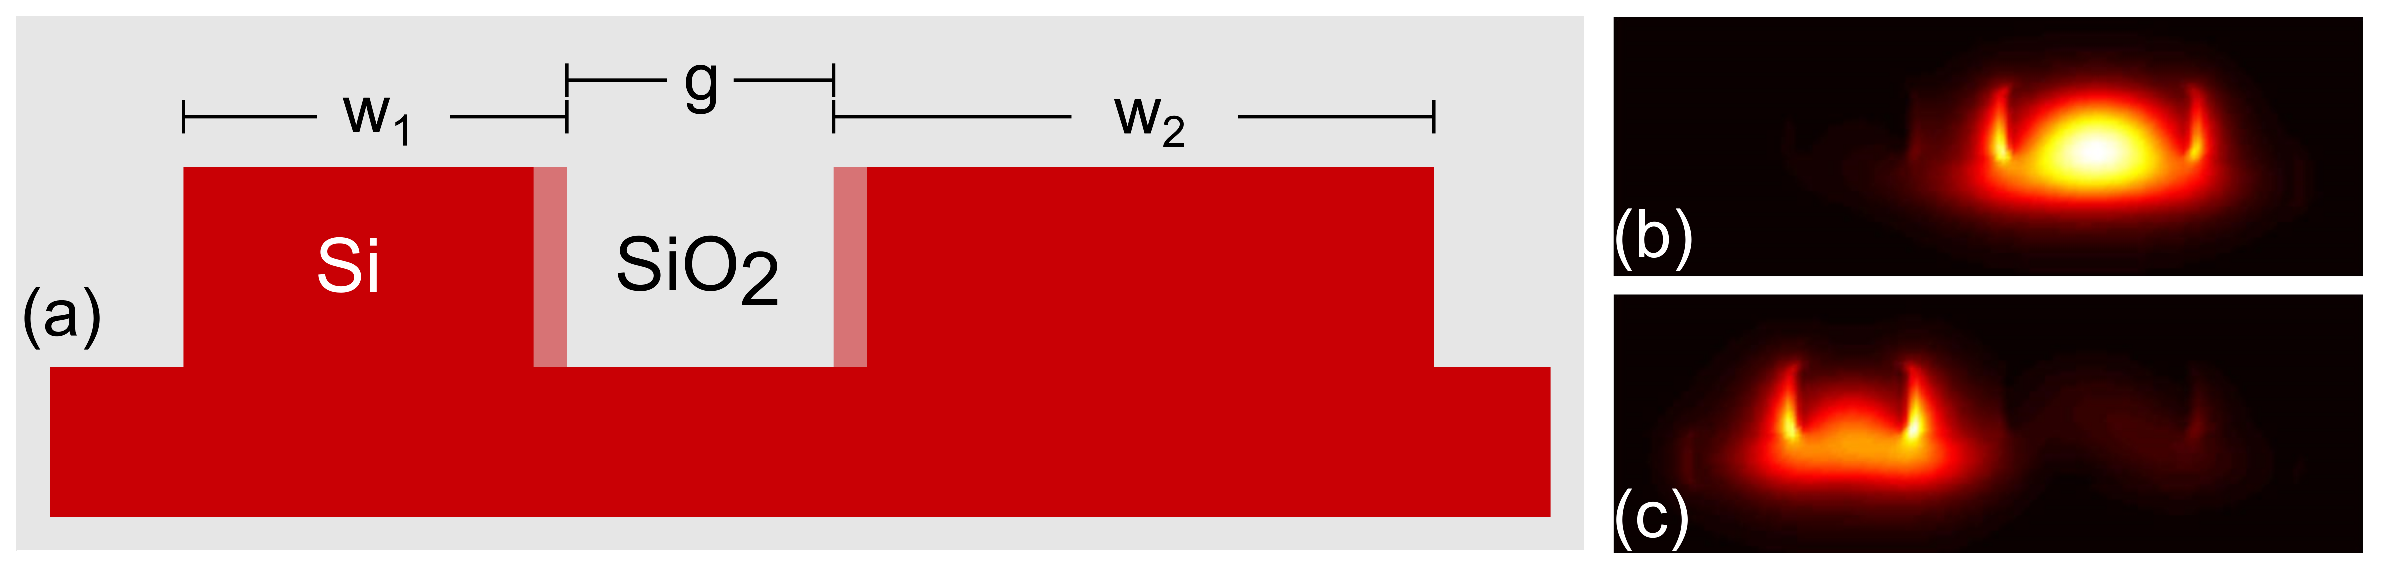
\includegraphics[width=.99\columnwidth]{CrossSection2}
	\caption{ a)Schematic cross-section: The contra-directional coupler is made of two silicon waveguides of different widths $w_1$ and $w_2$ with an average gap $g$ in-between them. The gap varies along the propagation axis. b) and c) Power distribution of the first and second supermode in the slab+contra-DC structure. }
	\label{fig:Device}
\end{figure}

The contra-directional coupler consists of two waveguides in close proximity, with a periodic change to the gap in-between them. This causes a wavelength selective contra-directional coupling at  $\lambda_\text{c} = \Lambda (n_\text{1}+n_\text{2})$, where $\Lambda$ is the grating pitch, and $n_\text{1}$ and $n_\text{2}$ are the effective refractive indices of the first-order and second-order eigenmodes in the coupler. 
The waveguides are highly asymmetric to suppress the co-directional coupling that would occur with two identical waveguides.

Figure \ref{fig:Device} shows the proposed cross-section of the waveguides in the coupling region. We observe that the modes are only weakly confined to the waveguides due their small widths (220 nm and 360 nm) and the slab; and that there is a strong overlap with the sidewalls of the grating. This bigger overlap allows us to design contra-DCs with a stronger coupling which reduces the loss and enables larger bandwidth.

The contra-DCs are apodized to reduce side-lobes, with the coupling following a gaussian profile with $a=10$ as described in \cite{shi2013siliconContraDC}.


\subsection{Fabrication process}
The fabrication process is a CMOS compatible deep UV (193 nm) lithography. The process uses a phase shifted mask as described in [CITE PHASE SHIFTED] which allows greater precision to resolve small features such as grating corrugations.

\subsection{Experiment}
Figure \ref{fig:litho} a) shows the test structure used to characterize 
\todo{Clear corrugations and the possibility to have a small gap under 140 nm.}
\begin{figure}[htbp]
	\centering
	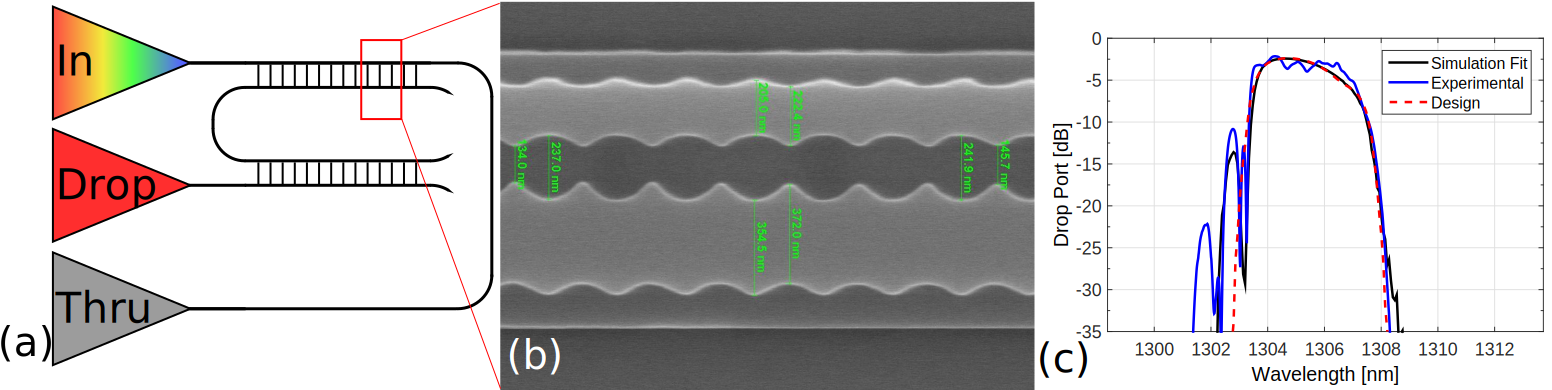
\includegraphics[width=.99\columnwidth]{SingleFilterFig}
	\caption{ a)Test structure b)SEM picture of a strong grating. The measurements show that the widths of the waveguides are not the same in the close and far region, resulting in a strong change of index along the propagation direction and a distortion of the apodization profile. c) Spectral response of the dual stage contra-DC filter, with simulation fit. }
	\label{fig:litho}
\end{figure}

\subsection{Filter optical performance}
Figure \ref{fig:litho} c) shows the spectral response of a dual stage filter. The insertion loss is 2.5 dB, the bandwidth covers 370 GHz and the sidelobes suppression is 8 dB. This weak sidelobes suppression is explained by the fact that strong corrugations are uneven on both sides, causing the effective index to be higher in the strong coupling regions than in the low coupling regions, which creates coupling dependent chirp; an different wavelength Bragg-condition along the grating. 

This coupling dependent chirp is considered in the simulation fit, which agrees with experimental results. With this information, we will be able to bias future devices to cancel this effect and create even gratings despite lithography distortion.

\subsection{WDM performance}
We see in figure \ref{fig:WDM} the response of the filter using a single filtering stage and also for two filtering stages.
\begin{figure}[htbp]
	\centering
	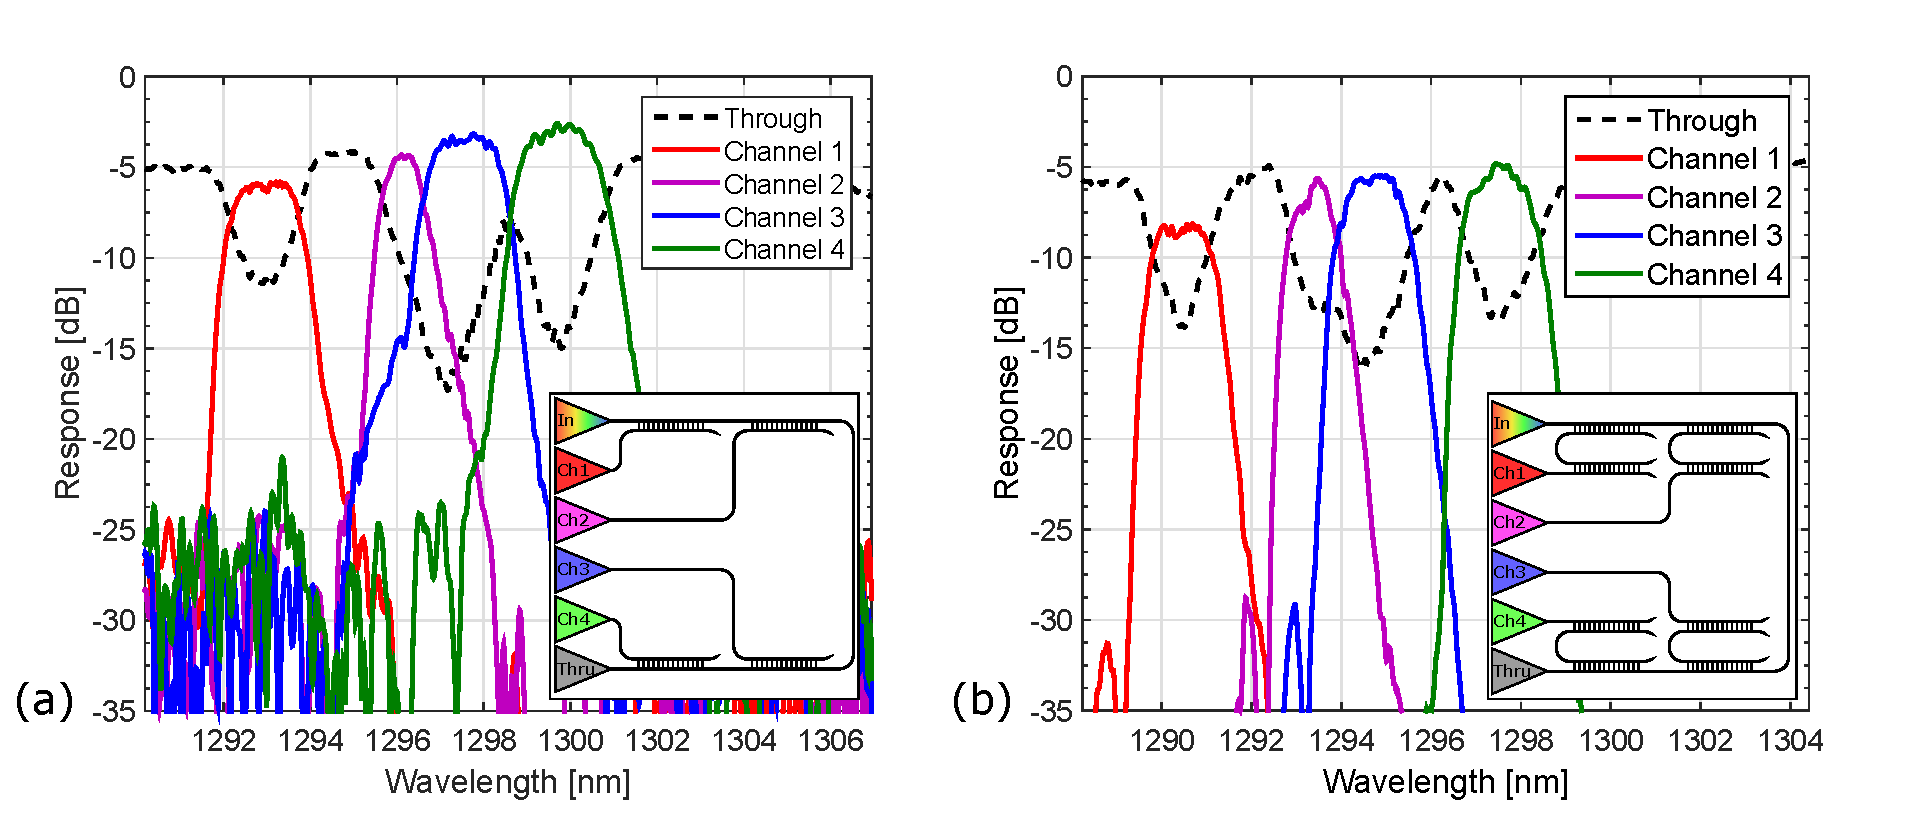
\includegraphics[width=.99\columnwidth]{WDM}
	\caption{a) Single stage WDM. b) Double staged WDM }
	\label{fig:WDM}
\end{figure}

Figure \ref{fig:WDM} shows the performance of four serial filters when used for WDM, for single stage and dual stage filtering. The way the channels differ is that they all have slightly different pitch $\Lambda$. Also, the channels are dropped in reverse order such that channel 3 has precedence over channel 2. This also explains why smaller channel numbers experience an higher loss, they have a longer optical path through more devices.

One obvious defect is that the second channel is smaller and offset. This is a systematic glitch in all the devices we measured, caused by the fact that channel 2 has an even grating pitch of 260 nm and that the grid resolution of the fabrication is 1 nm, causing it to snap differently to the grid then the other devices. This causes its central wavelength to be slightly higher.




\section{Conclusion}
\todo{The demonstrated device open possibilities for wide bandwidth and temperature tolerant filters with a flat top response. Next prototypes promise to offer even larger bandwidth and a more square shape after biasing for lithography.}













\section*{Acknowledgments}
We acknowledge CMC Microsystems for the  software and the fabrication subsidy. The authors acknowledge the Natural Sciences and Engineering Research Council of Canada for funding this research. This work is part of the SPEED research project (Silicon Photonic Electrically Engineered Devices) funded by NSERC (RDCPJ438811-12), PROMPT (PJT-2011-17), and TeraXion.

\bibliographystyle{osajnl}
\bibliography{bibli}

\end{document}